\documentclass[paperwidth=40in,paperheight=32in,landscape]{baposter} % Set poster size and orientation

\usepackage{amsmath,amssymb}
\usepackage{graphics}
\graphicspath{{images/}}
\usepackage{color}
\usepackage{multicol}
	\setlength{\columnseprule}{1pt}
	\def\columnseprulecolor{\color{black}}

\usepackage{enumitem}
	
\newcommand{\headshotsize}{0.95in}
\newcommand{\logosize}{0.75in}
% \newcommand{\headshotsize}{1.0in}
%%% Color Definitions %%%

\definecolor{cuGold}{cmyk}{0, .10, .48, .22}
\definecolor{cuBlack}{cmyk}{0, 0, 0, 1.00}
\definecolor{cuDarkGray}{cmyk}{.38, .28, .21, .63}
\definecolor{cuLightGray}{cmyk}{.16, .11, .11, .29}

\definecolor{bordercol}{RGB}{0,0,0} % Content cell border color
\definecolor{headercol}{RGB}{229,240,241} % Concent cell header fill color
\definecolor{headerfontcol}{RGB}{0,0,0} % Concent cell header text color
\definecolor{boxcol}{RGB}{255,255,255} % Concent cell background color

% Custom commands
\newcommand{\RR}{\mathbb{R}}
\newcommand{\NN}{\mathbb{N}}
\newcommand{\OO}{\mathcal{O}}
\newcommand{\mathcow}{\OO}
\newcommand{\QQ}{\mathbb{Q}}
\newcommand{\ZZ}{\mathbb{Z}}
\newcommand{\CC}{\mathbb{C}}
\newcommand{\KK}{\mathbb{K}}
\newcommand{\PP}{\mathcal{P}}
\newcommand{\TT}{\mathcal{T}}
\newcommand{\BB}{\mathcal{B}}
\newcommand{\LL}{\mathcal{L}}
\renewcommand{\Re}{\operatorname{Re}}
\renewcommand{\Im}{\operatorname{Im}}

\newcommand{\veca}{\vec{a}}
\newcommand{\vecb}{\vec{b}}
\newcommand{\vecd}{\vec{d}}
\newcommand{\vece}{\vec{e}}
\newcommand{\vecf}{\vec{f}}
\newcommand{\vecn}{\vec{n}}
\newcommand{\vecp}{\vec{p}}
\newcommand{\vecr}{\vec{r}}
\newcommand{\vecu}{\vec{u}}
\newcommand{\vecv}{\vec{v}}
\newcommand{\vecw}{\vec{w}}
\newcommand{\vecx}{\vec{x}}
\newcommand{\vecy}{\vec{y}}
\newcommand{\vecz}{\vec{z}}

\renewcommand{\vec}[1]{\mathbf{#1}}
\newcommand{\norm}[1]{\left\lVert #1 \right\rVert}

%%% Document Start %%%

\begin{document}

%%% Poster Settings %%%

\begin{poster}{
	grid = false, % Turns off alignment grid 
	columns = 4, % Sets number of poster columns
	colspacing = 1em,
	headerheight = 0.1\textheight,
	background = plain,
	bgColorOne = cuBlack,
	borderColor = cuGold,
	headerColorOne = cuDarkGray,
	textborder = rounded,
	headerborder = closed,
	headershape = rounded,
	headershade = plain,
	boxshade = plain,
	headerfont = \Large\sf\bf,
	headerFontColor = cuGold,
	boxColorOne = white,
	linewidth = 2pt
}
{

\includegraphics[height=\logosize, trim={0.5cm, 1cm, 16.4cm, 0.7cm}, clip=true]{cu_logo}
\hspace{.3cm}
\includegraphics[height=\logosize]{NSF_logo.eps}
\hspace{.3cm}

\includegraphics[height=\logosize]{qrcode.png}
\hspace{.3cm}
}
{\sf\bf
	\color{cuGold}
	RBF Quadrature for Neural Fields
}
{
	\color{cuGold}
	Sage B. Shaw$^{1}$, Zachary P. Kilpatrick$^1$, and Daniele Avitable$^2$\\
	\small{1: University of Colorado Boulder}
	\small{2: Vrije Universiteit Amsterdam}
}
{
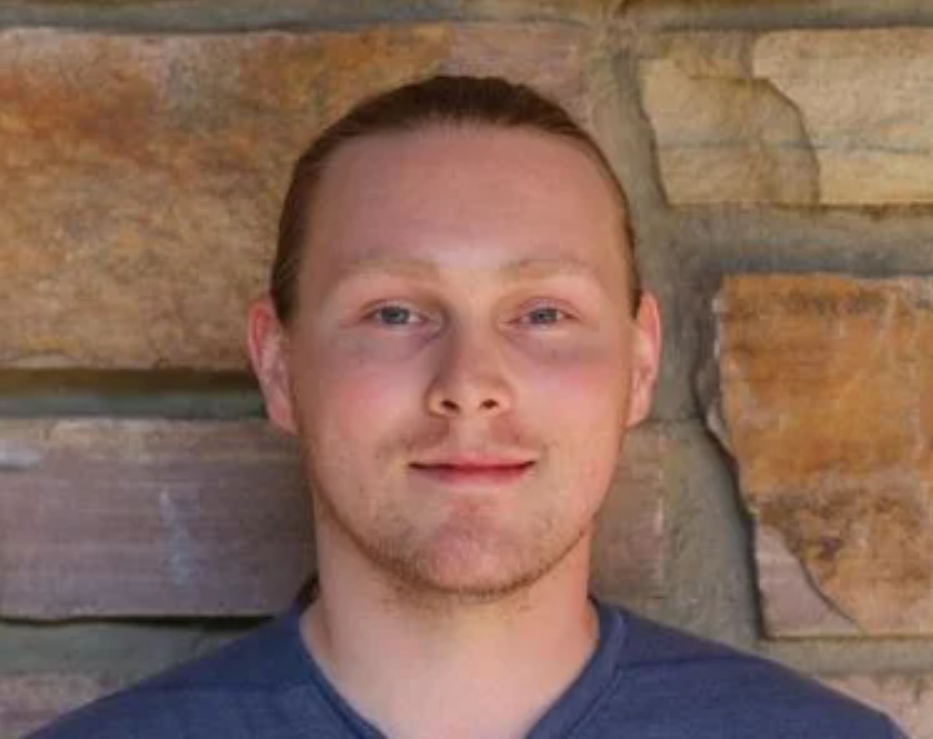
\includegraphics[height=\headshotsize, trim={3cm, 0cm, 3cm, 0cm}, clip=true]{headshot_sage}
\hspace{.5cm}
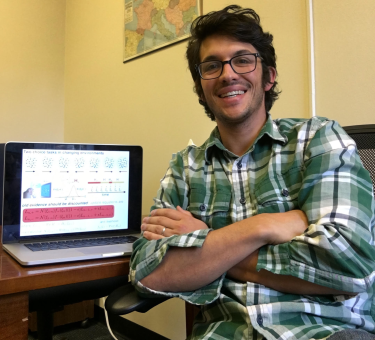
\includegraphics[height=\headshotsize, trim={5.1cm, 6cm, 2cm, 0cm}, clip=true]{headshot_zack}
\hspace{.5cm}
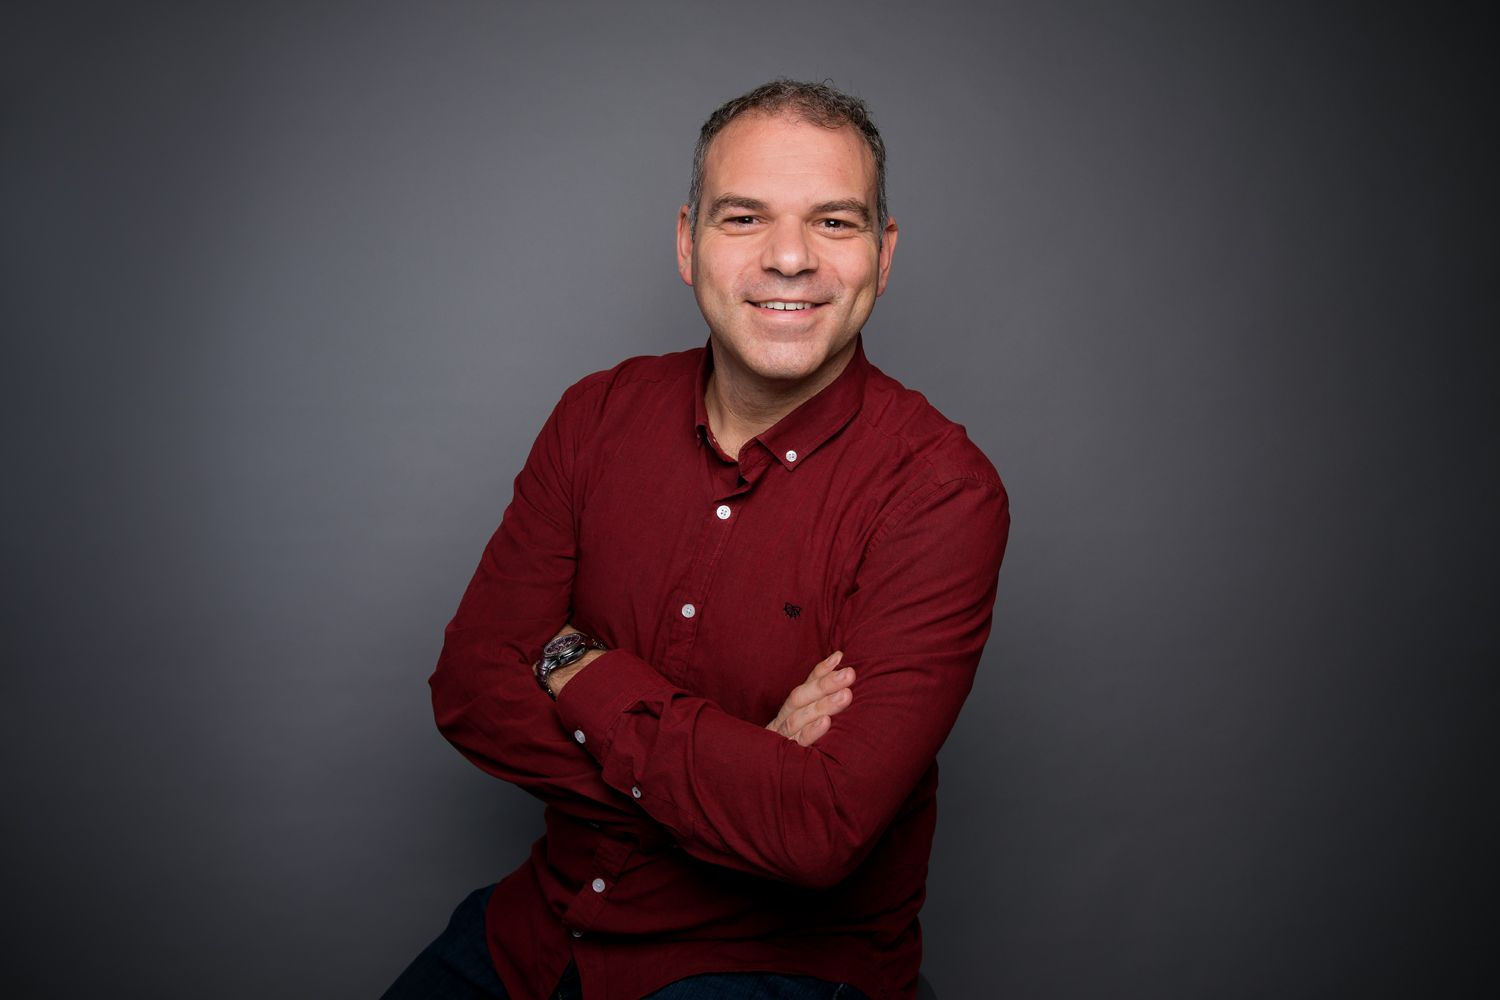
\includegraphics[height=\headshotsize, trim={21cm, 20cm, 18cm, 2cm}, clip=true]{headshot_daniele}
}
%%% Poster Content %%%

%%%%%%%%%%%%%%%%%%%
%%% Column 0
%%%%%%%%%%%%%%%%%%%
\headerbox{Summary}{name = summary, column = 0}{
	\textbf{Goal:} To create and test a neural field solver using radial basis function quadrature.
	The method should be
	\vspace{-.5em}
	\begin{itemize}[leftmargin=*]
		\setlength\itemsep{-.5em}
		\item High-order accurate
		\item Stable
		\item Geometrically flexible
		\item Fast (low complexity)
	\end{itemize}
	\vspace{-.5em}
	In the future, we will extend this to realistic curved 2D spatial domains.
}

\headerbox{Neural Field Models (NF)}{name = neuralfield, column = 0, below=summary}{
	\begin{itemize}[leftmargin=*]
		\setlength\itemsep{-.2em}
		\item Tissue level models
		\item Integro-differential equation(s)
		\item Integral kernel represents neural network connectivity
		\item Non-linear firing rate function captures non-linear neural dynamics
	\end{itemize}
	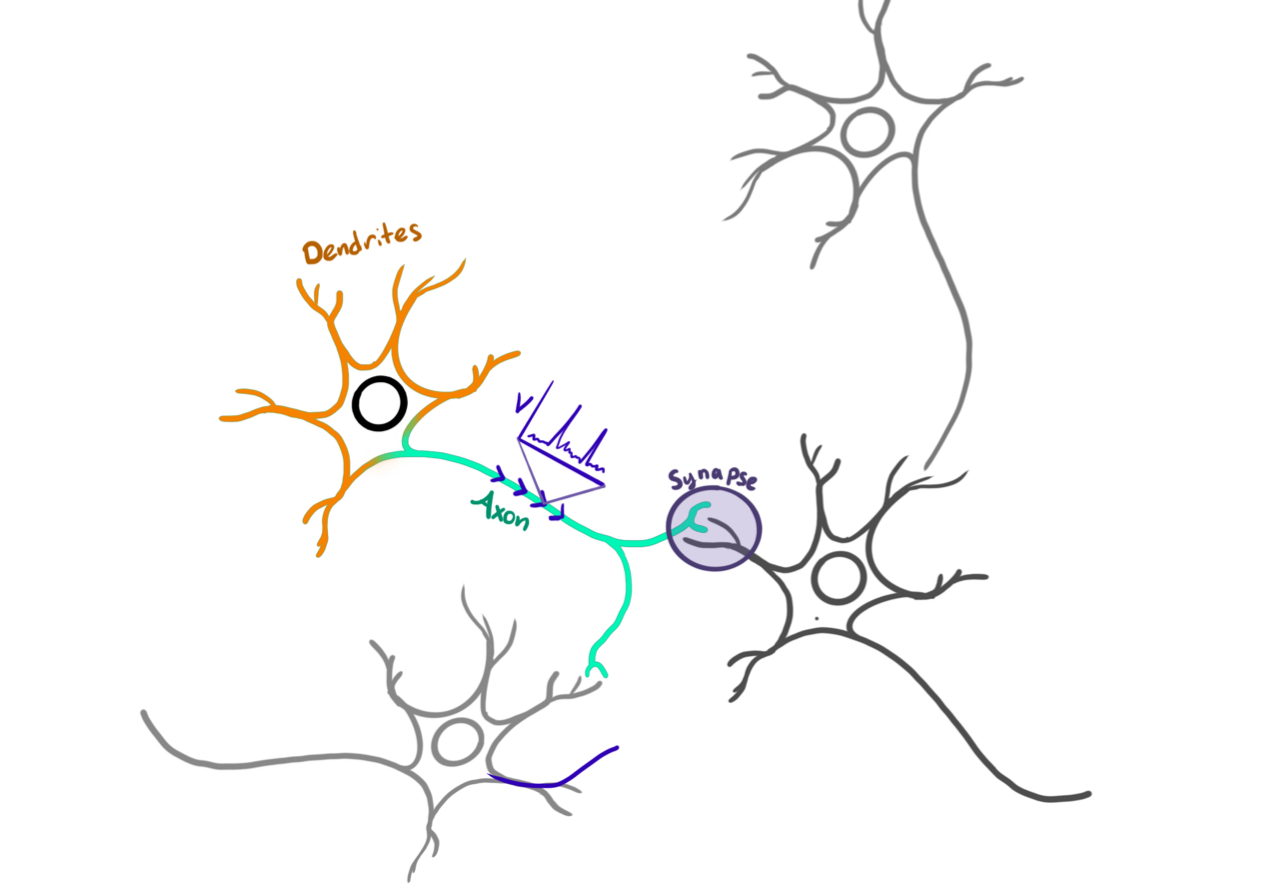
\includegraphics[width=\linewidth, clip=true, trim={0cm, 7cm, 0cm, 7cm}]{images/neurons}
	\centerline{\small Image by Dr. Heather Cihak.} \\
	\vspace{-.2em}
	$\partial_t u(t, \vecx) = -u + \iint_\Omega w(\vecx, \vecy) f[u(t, \vecy)] \ d\vecy$
	\begin{itemize}[leftmargin=*]
		\setlength\itemsep{-.2em}
		\item $u(t, \vecx)$ --- Neural activity
		\item $w(\vecx, \vecy)$ --- Connectivity kernel
		\item $f(\cdot)$ --- Non-linear firing rate function
		\item $\Omega = [0, 1]^2$ for now.
	\end{itemize}
	\vspace{-1.5em}
	\begin{center}
		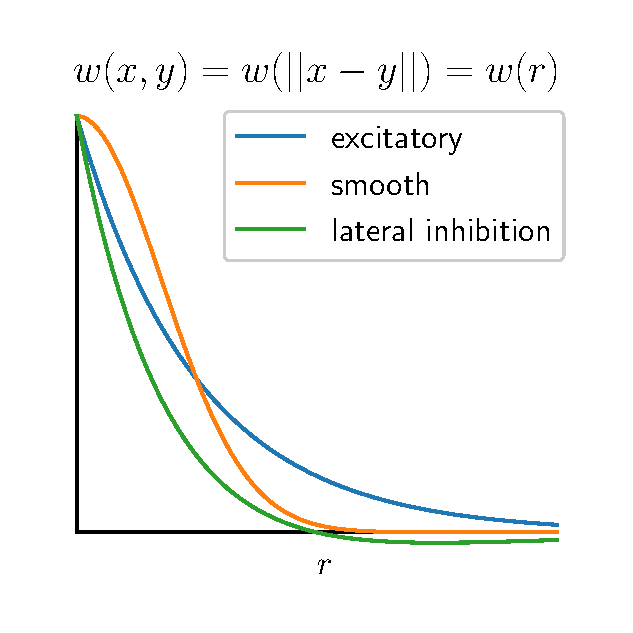
\includegraphics[width=.9\linewidth, trim={0cm, .13cm, 0cm, 0cm}, clip=true]{images/kernels}
	\end{center}
}

%%%%%%%%%%%%%%%%%%%
%%% Column 1 
%%%%%%%%%%%%%%%%%%%
\headerbox{$\begin{array}{l}
\text{Radial Basis Function}\\ \text{Quadrature Formuale}
\end{array}$
}{name = rbfqf, column = 1, boxheaderheight=1.3cm}{
	% Itemize Example:
	\begin{itemize}[leftmargin=*]
		\setlength\itemsep{-.4em}
		\item Abreviated \textbf{RBF-QF}
		\item Place $N$ nodes in $\Omega$
		\item Partition $\Omega$ into elements
		\item For each element
		\vspace{-1em}
		\begin{itemize}
			\setlength\itemsep{-.2em}
			\item Select the $k$ nearest nodes \\(the stencil),
			\item Interpolate Lagrange functions,
			\item Integrate over the element,
			\item Sum over interpolants
		\end{itemize}
		\setlength\itemsep{-1em}
		\item Sum over elements
	\end{itemize}
	\vspace{-0.5em}
	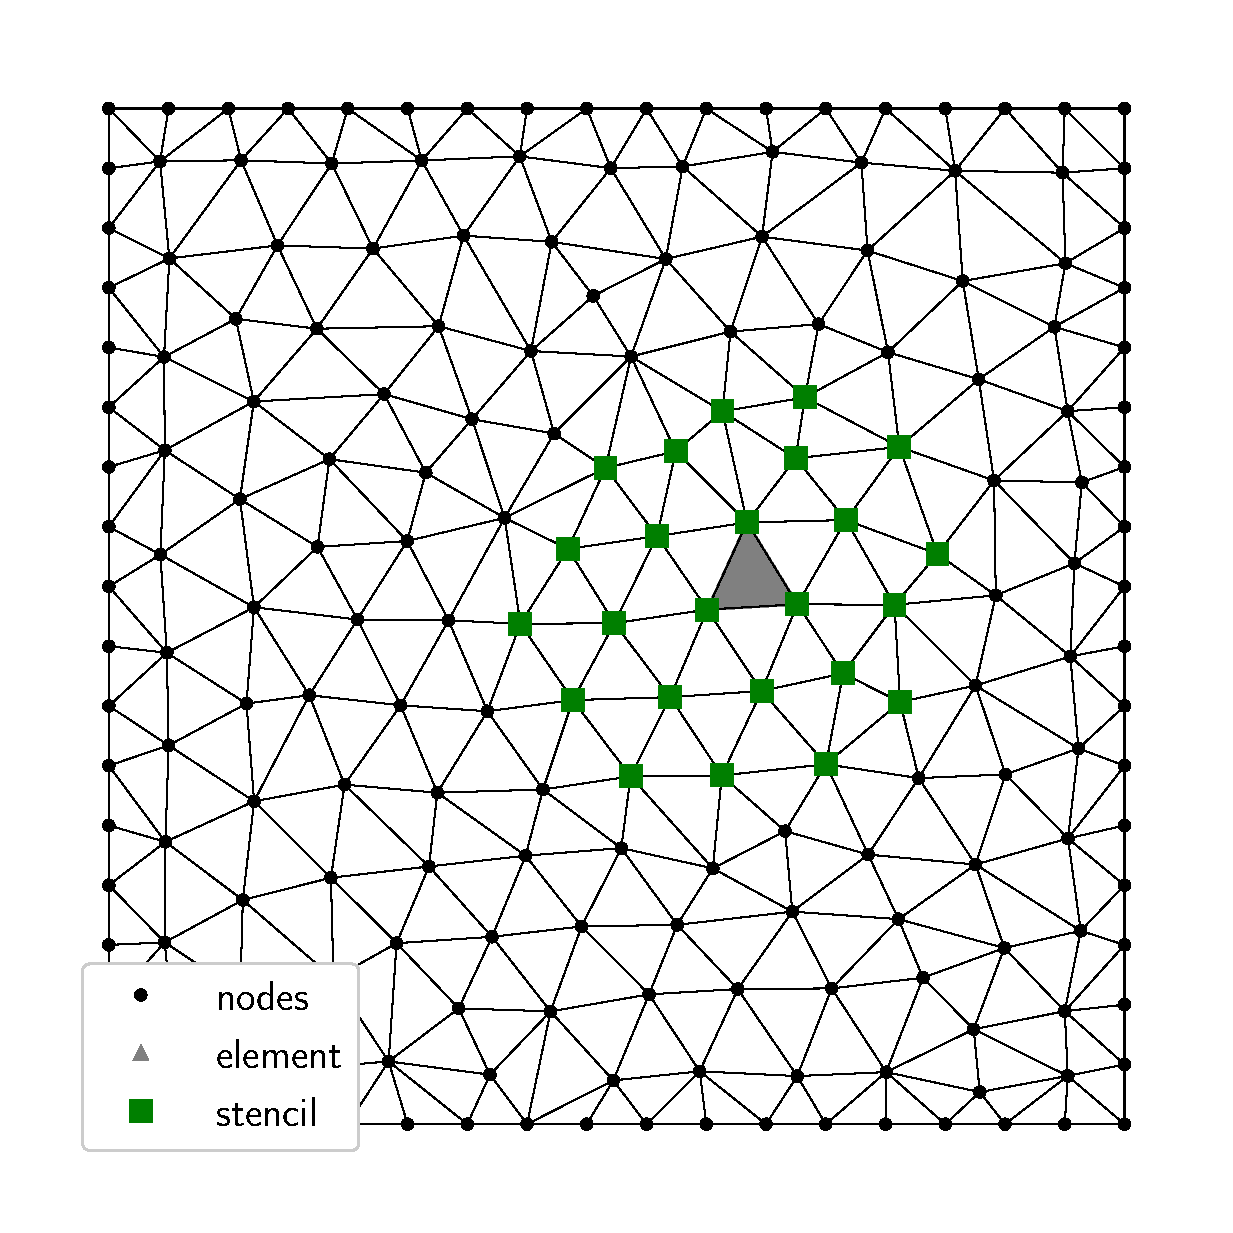
\includegraphics[width=\linewidth, trim={0cm, 1.1cm, 0cm, 1.4cm}, clip=true]{images/triangulation}
	The local interpolants have the form
	\vspace{-0.5em}
	\[
		s(\vecx) = \sum_{i=1}^k c_i \phi(\norm{\vecx - \vecx_i}) + \sum_{j=1}^m \gamma_i \pi_j(\vecx)
	\]
	\vspace{-2em}
	\begin{itemize}[leftmargin=*]
		\setlength\itemsep{-.4em}
		\item $\phi$ - radial basis function \\
		(eg. $\phi(r) = r^3$)
		\item $\{\pi_{j}\}_{j=1}^m$ - polynomial basis
		\item $k$ interpolation conditions
		\item $m$ moment conditions
	\end{itemize}
	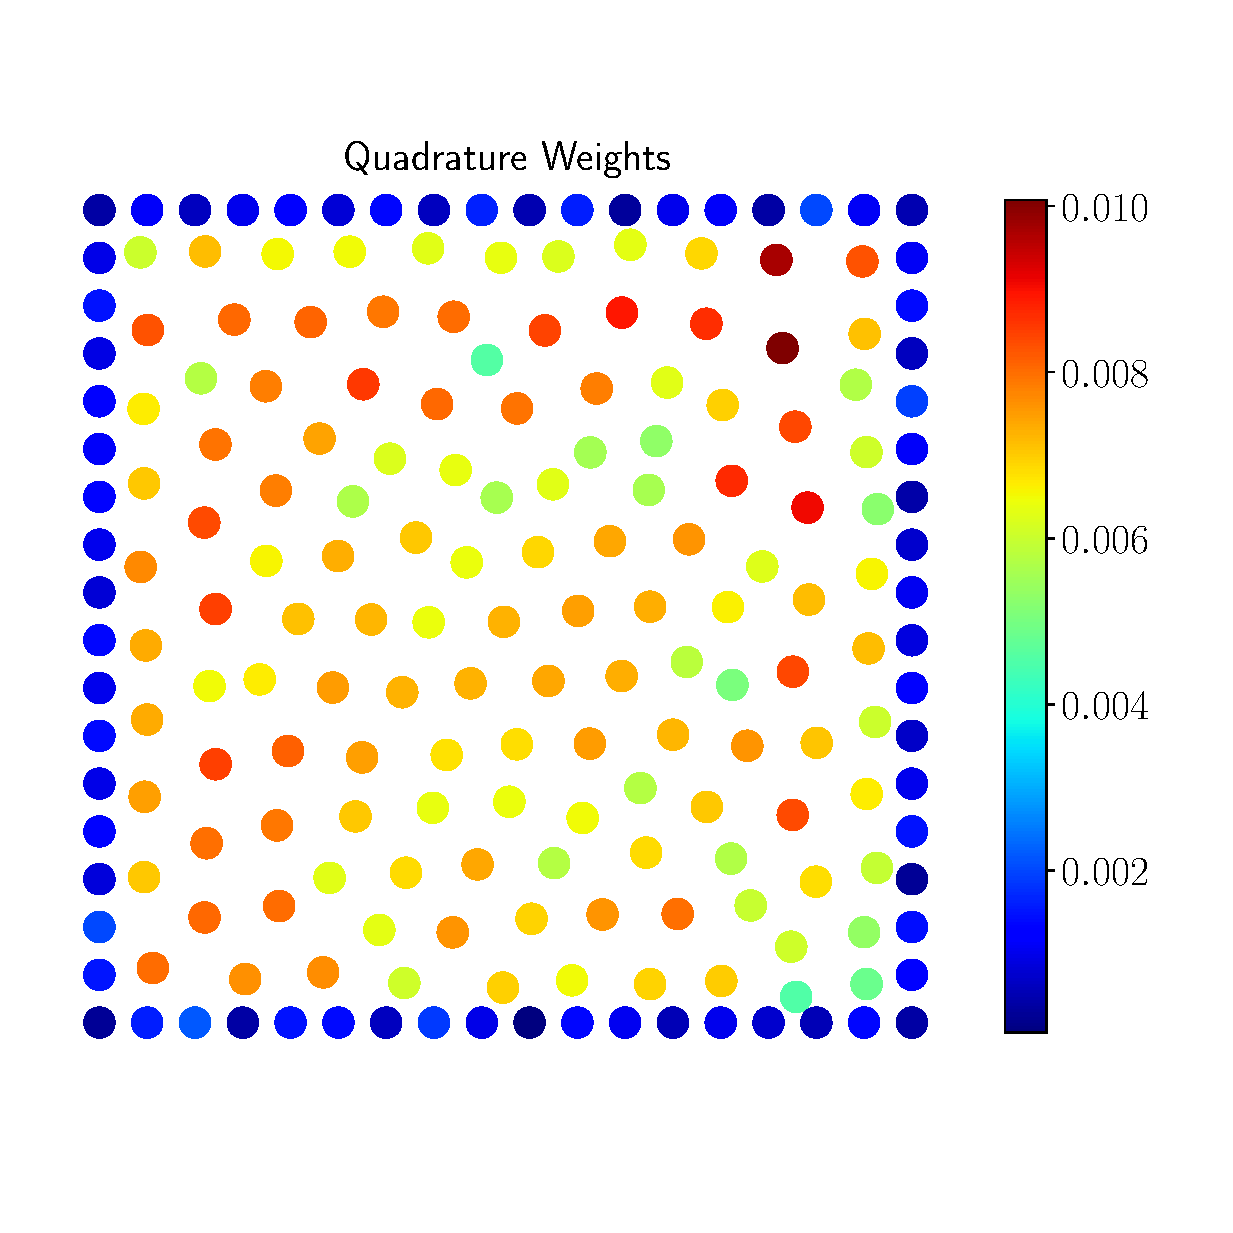
\includegraphics[width=\linewidth, trim={0cm, 3cm, 0cm, 2cm}, clip=true]{images/weights}
	\vspace{-.3cm}
}

%%%%%%%%%%%%%%%%%%%
%%% Column 2
%%%%%%%%%%%%%%%%%%%
\headerbox{Quadrature Convergence}{name = quad_convergence, column = 2}{
	\begin{itemize}[leftmargin=*]
		\setlength\itemsep{-.1em}
		\item No proven convergence rate.
		\item We expect at least $\mathcal{O}(d+1)$, where $d$ is the degree of polynomial basis. \\(Think trapezoidal rule.)
		\item We test this on a product of Chebyshev polynomials.
		\item Area per point scaleds like $\mathcal{O}(N^{-1/2})$
	\end{itemize}
	\begin{center}
		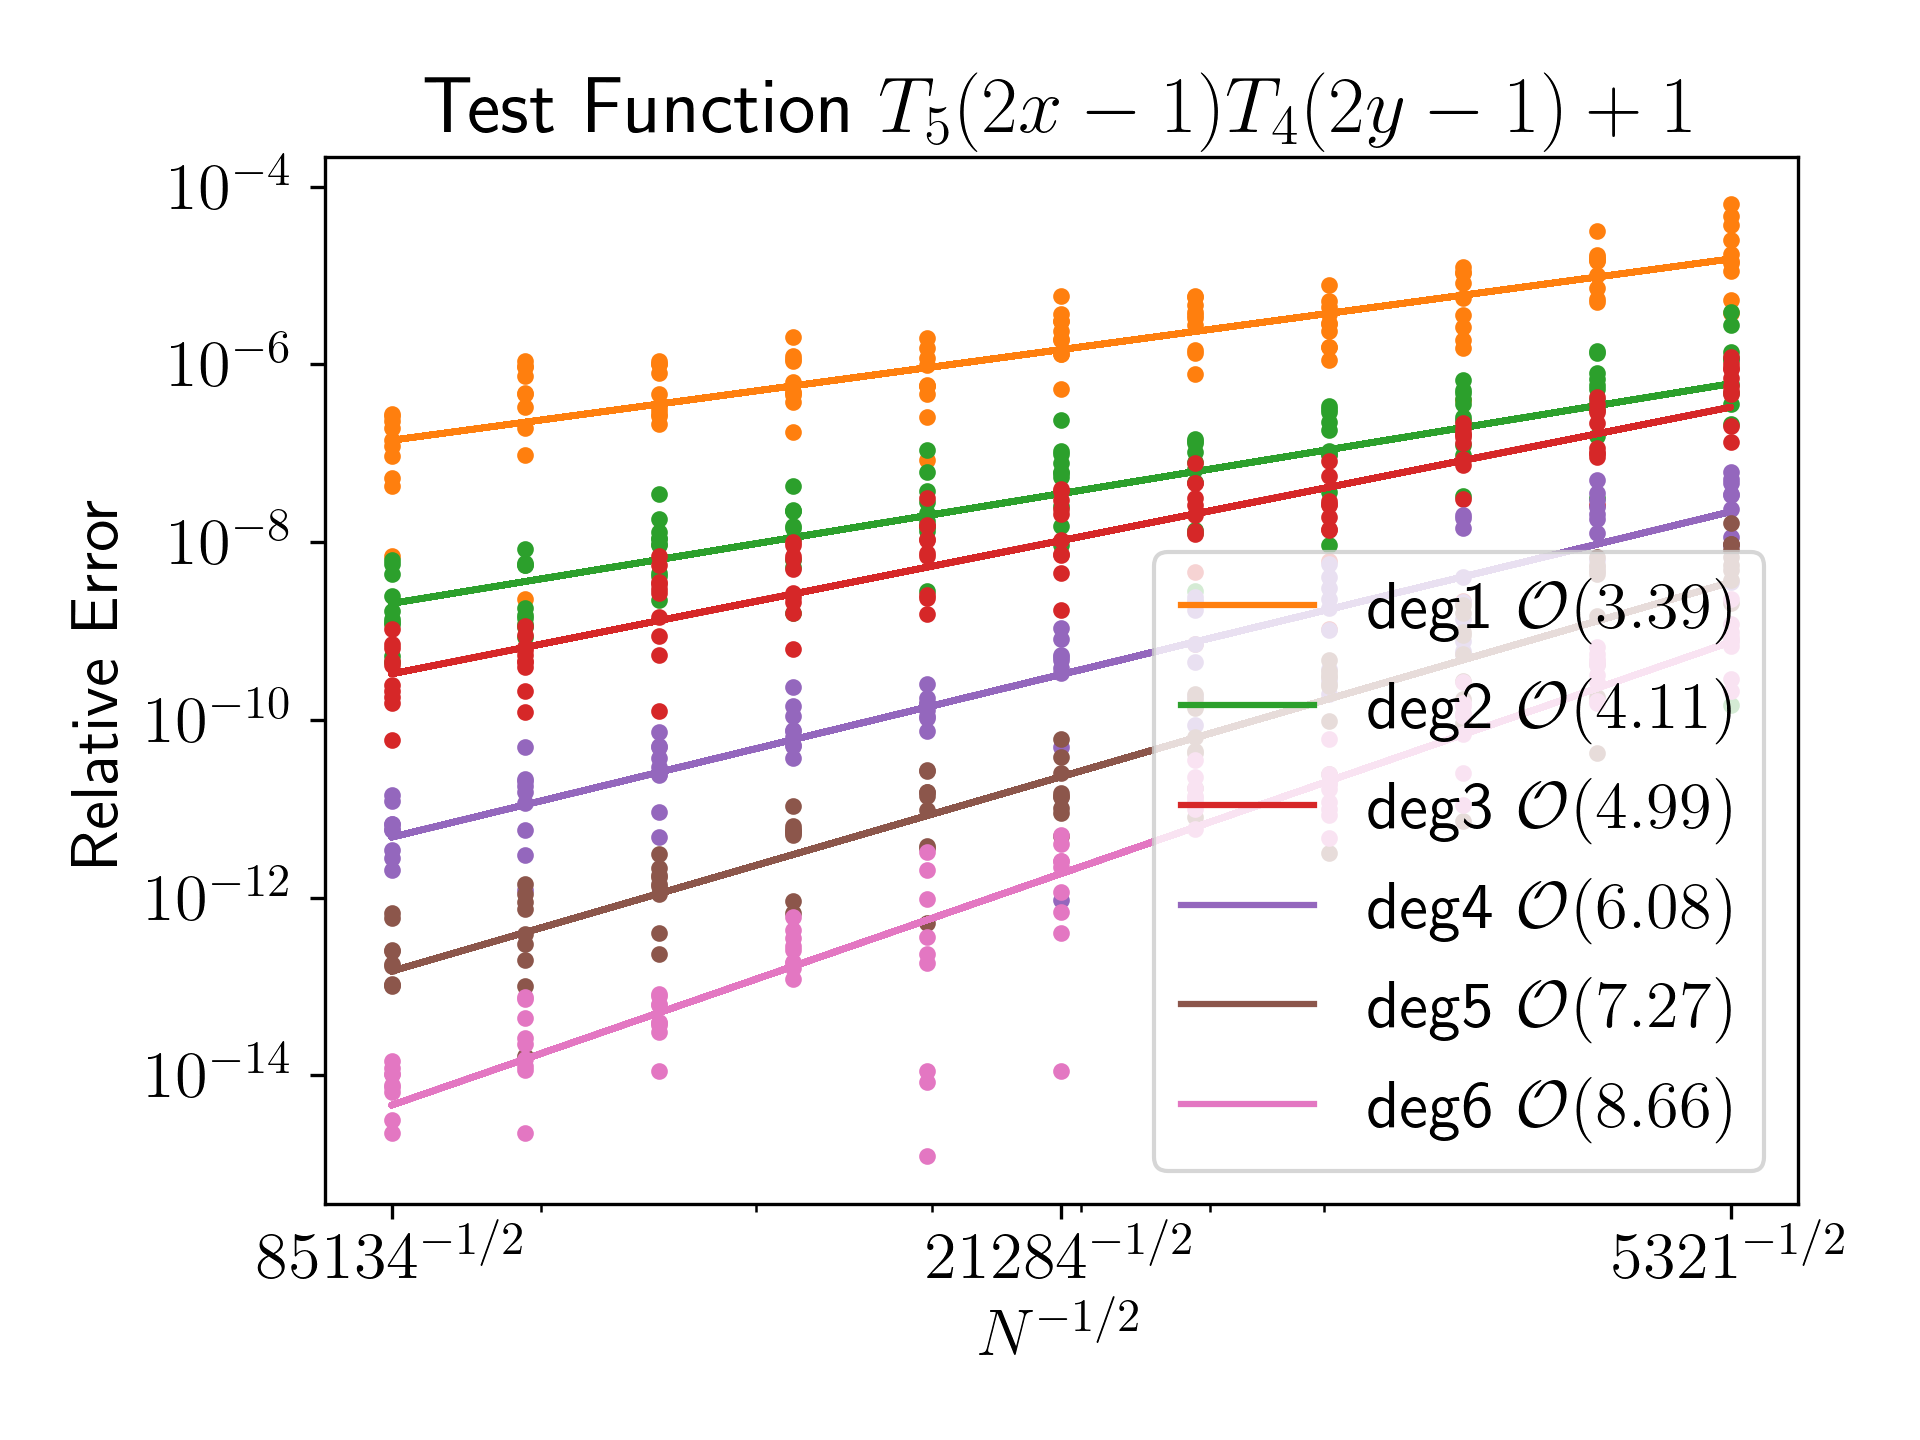
\includegraphics[width=\linewidth, clip=true, trim={.5cm, 0cm, .5cm, 0cm}]{images/quad_convergence}
	\end{center}
	\vspace{-2em}
	\begin{itemize}[leftmargin=*]
		\setlength\itemsep{-.1em}
		\item Better convergence than expected
	\end{itemize}
}

\headerbox{Spatial Analysis}{name = quad, column = 2, below=quad_convergence}{
	\begin{itemize}[leftmargin=*]
		\setlength\itemsep{-.1em}
		\small
		\item Gaussian test functions centered at $(x_0, y_0)$
		\item Scattered Nodes vs Regular Hex Grid
	\end{itemize}
	\begin{center}
		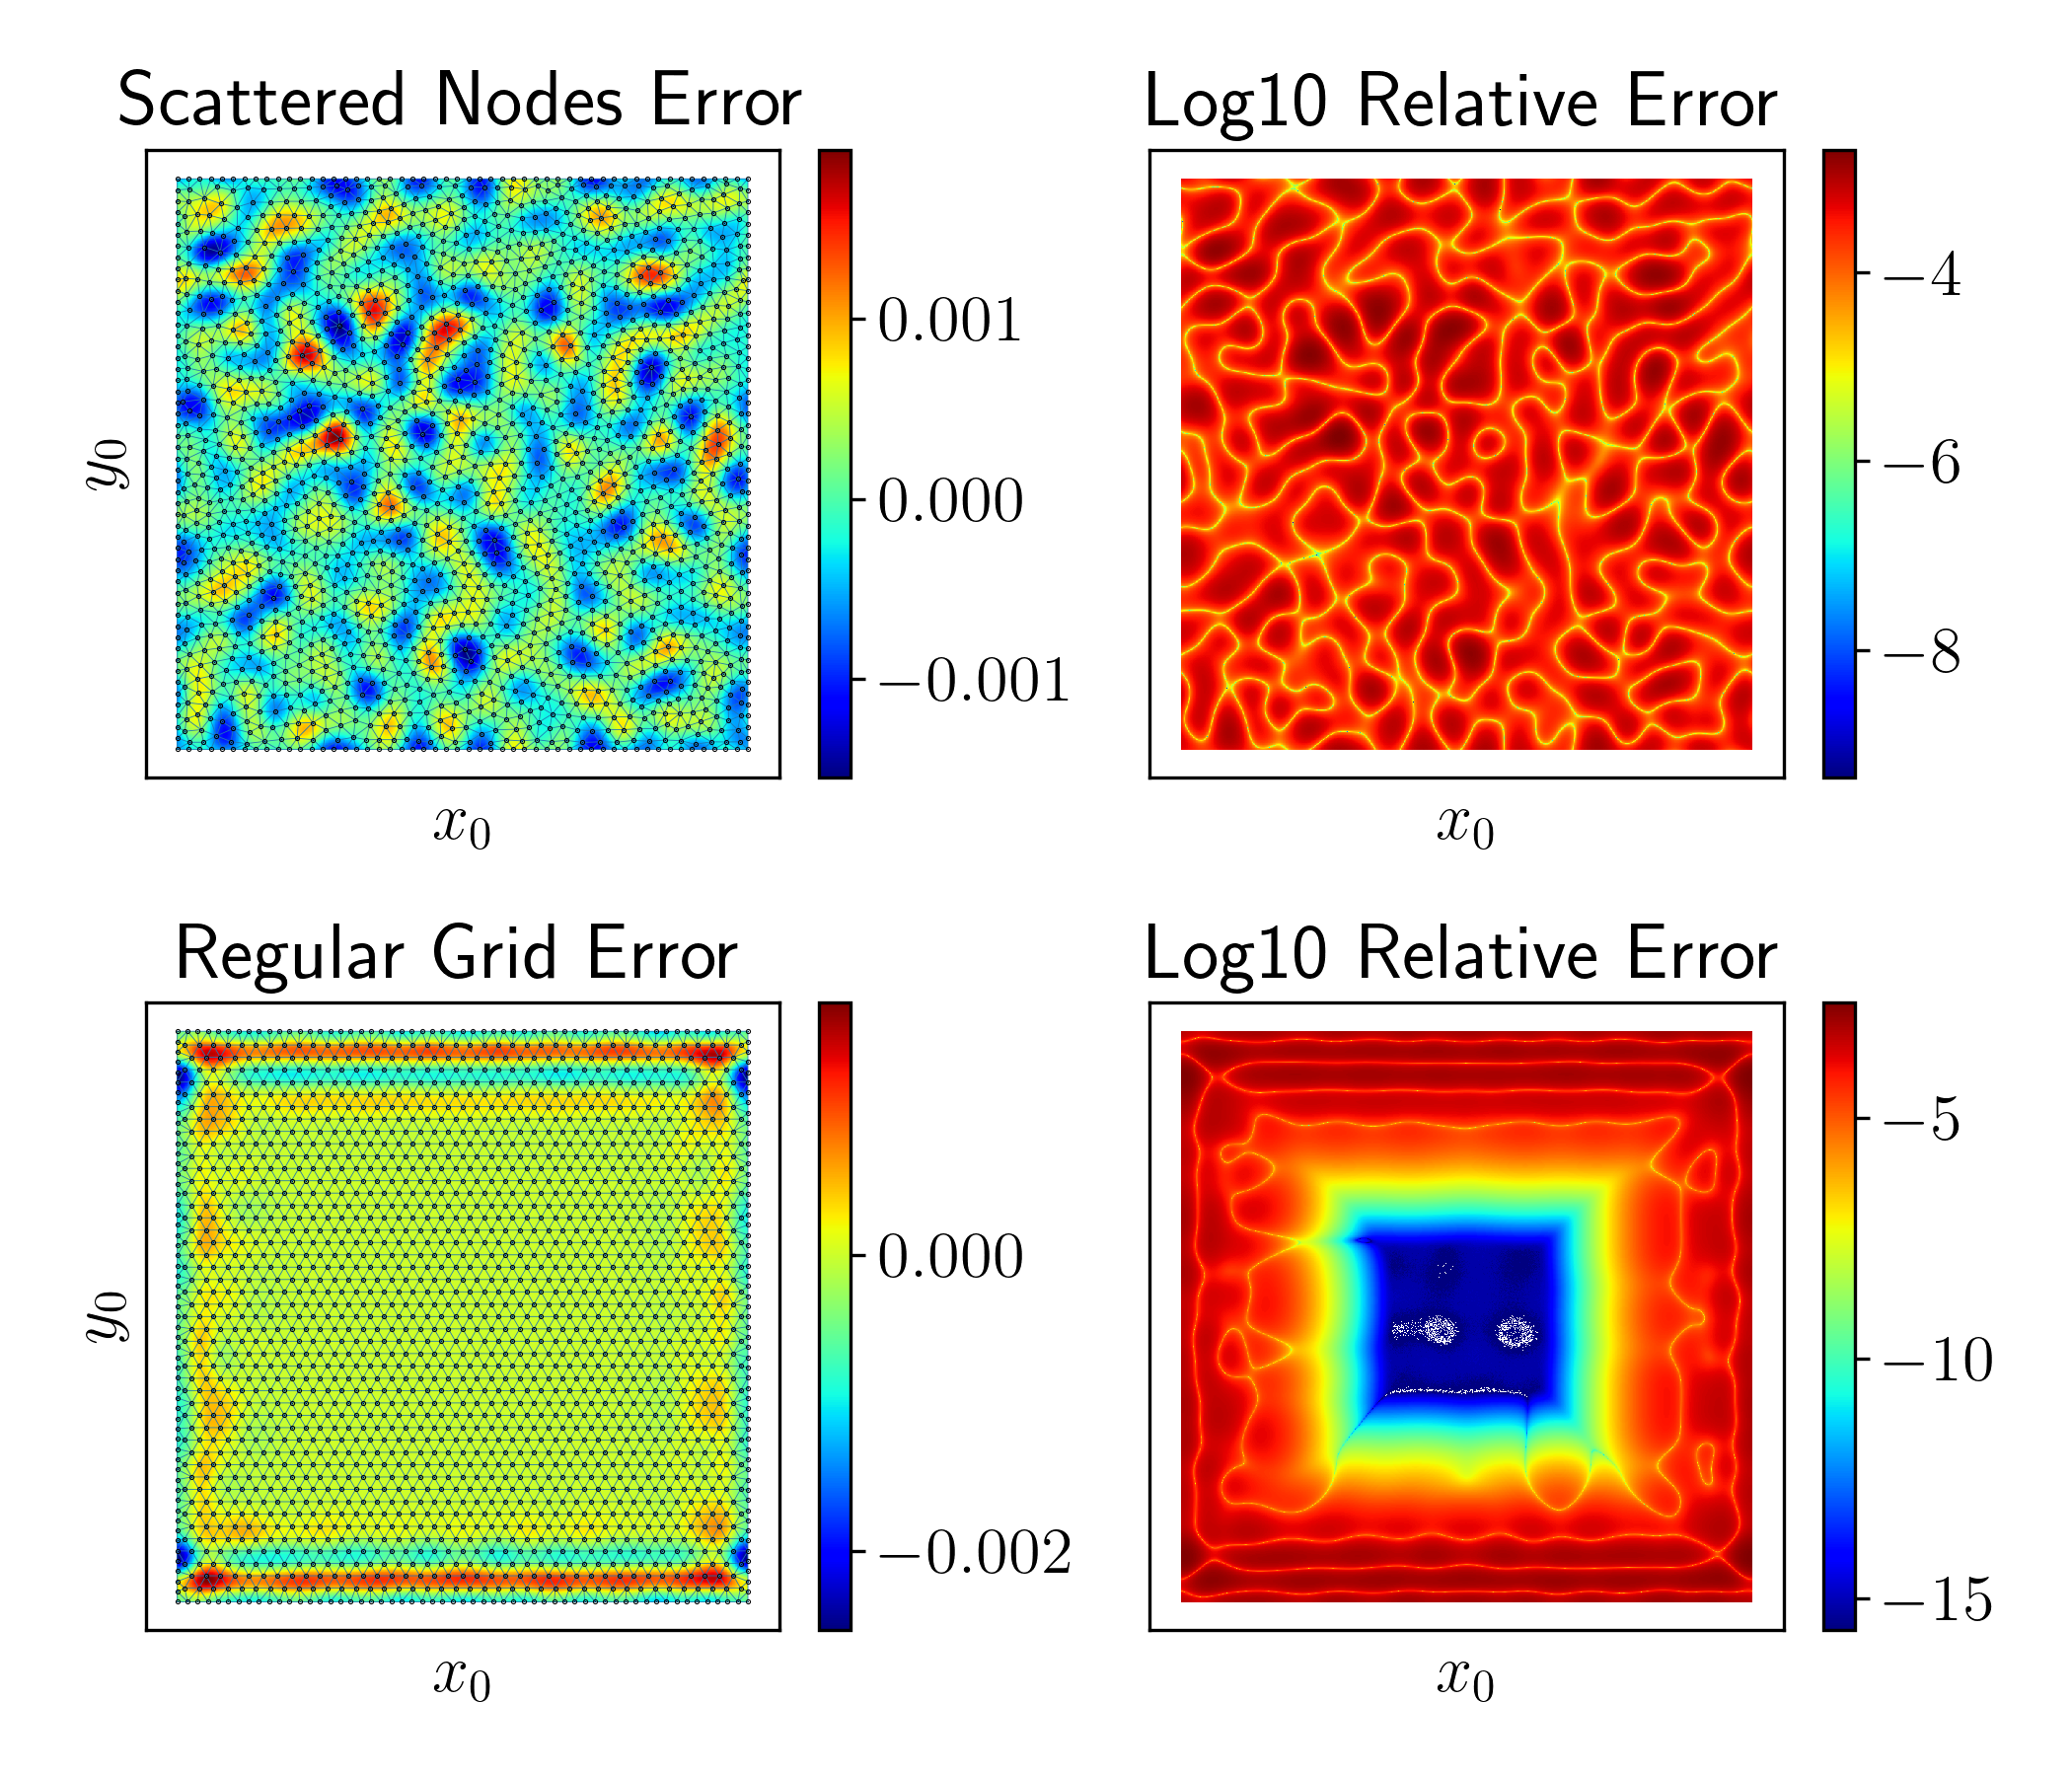
\includegraphics[width=\linewidth, trim={.5cm, .5cm, .5cm, 0cm}, clip=true]{images/poster_space_combined}
	\end{center}
	\begin{itemize}[leftmargin=*]
		\setlength\itemsep{-.1em}
		\small
		\item Error is continuous w.r.t. $(x_0, y_0)$
		\item Hex grid has spectral accuracy away from boundary \\ (like trapezoidal rule)
	\end{itemize}
	\vspace{-.31cm}
}

%%%%%%%%%%%%%%%%%%%
%%% Column 3
%%%%%%%%%%%%%%%%%%%
\headerbox{Next Steps}{name = ivp, column = 3}{
	\vspace{-.2em}
	\textbf{Projection Method}[1] % Avitable
	\vspace{-.8em}
	\begin{itemize}[leftmargin=*]
		\setlength\itemsep{-.4em}
		\small
		\item Framework for error analysis of NF
		\item error = projection error + QF error
		\item We will unify these errors using RBF interpolation (projection) and RBF-QF.
	\end{itemize}
	\vspace{-.2em}
	\textbf{Curved 2D Manifolds}
	\vspace{-.8em}
	\begin{itemize}[leftmargin=*]
		\setlength\itemsep{-.2em}
		\small
		\item {[2,3]} Extended RBF-QF to 2D manifolds % Reeger
		\item {[4]} Used FitzHugh–Nagumo (toy model) on torrus (toy surface) to study effects of cortical curvature.
		\item We will use RBF-QF on realistic cortical surfaces
			 to study the effects of cortical curvature on \textit{cortical spreading depression} (CSD).
	\end{itemize}
	\vspace{-.2em}
	\textbf{Cortical Spreading Depression}
	\vspace{-.8em}
	\begin{itemize}[leftmargin=*]
		\setlength\itemsep{-.4em}
		\small
		\item Slow moving chemical wave
		\item Causes depressed neural activity
		\item Causes \textit{scintilating scotomas}
	\end{itemize}
	\vspace{-.5em}
	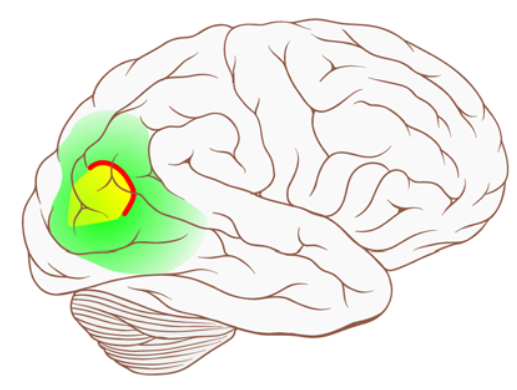
\includegraphics[width=0.9\linewidth, trim={0cm, .5cm, 0cm, 0cm}, clip=true]{images/csd}
	\begin{center} \small Cartoon of CSD wave[5]\end{center} % Dahlam
	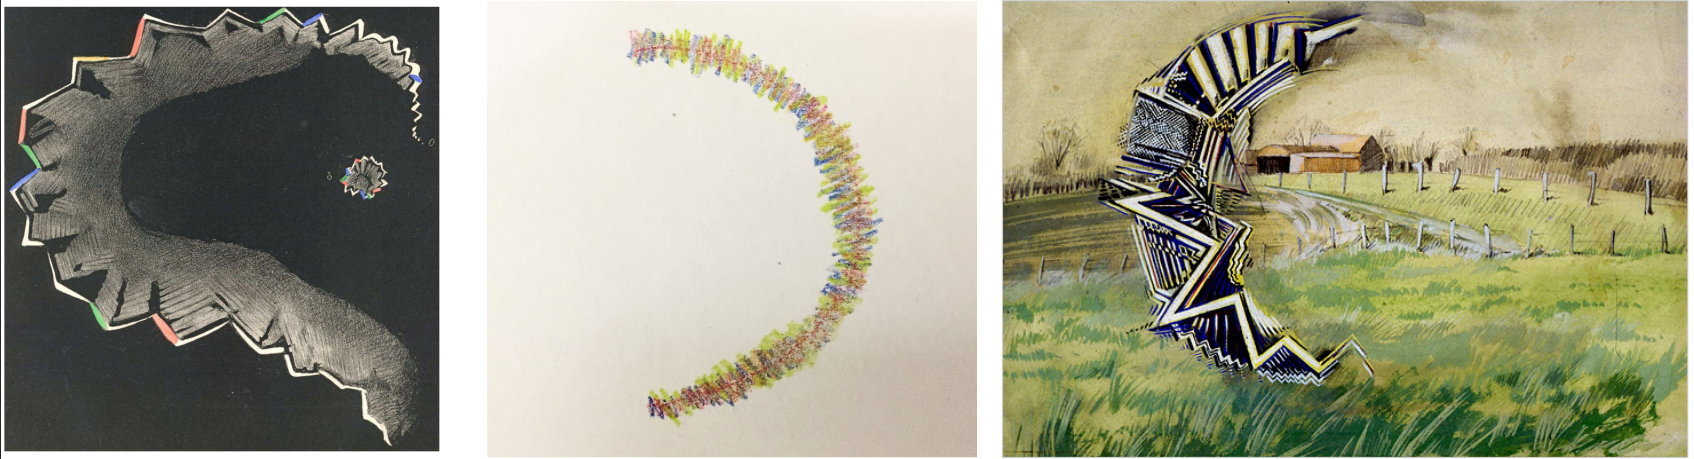
\includegraphics[width=\linewidth, trim={0cm, 0cm, 0cm, 0cm}, clip]{images/scotoma}
	\vspace{-2.2em}
	\begin{center} \small Artistic Rendering of Scotomas (see QR code)\end{center}
}

\headerbox{References and Funding}{name = ref, column = 3, below=ivp}{
	% Itemize Example:
	\begin{enumerate}[leftmargin=*]
		\setlength\itemsep{-.4em}
		\small{
			\item D. Avitable (2023) SIAM J. Numer. Anal. % projection paper
			\item Regeer et al. (2016) Proc. Royal A % smooth surfaces without boundary
			\item Reeger \& Fornberg (2018) J. Comp. Phys. % smooth surfaces with boundary
			\item Kneer et al. (2014) New Journal of Physics.
			\item M. Dahlam (2013) Chaos.
		}
	\end{enumerate}
	\vspace{-.75em}
	\texttt{shawsa.github.io/presentations} \\
	\small{This work is supported by} \\
	\small{NSF DMS-2207700} \\
	\small{NIH BRAIN 1R01EB029847-01}
	\vspace{.2em}
}

%%%%%%%%%%%%%%%%%%%%%%%%%%%%%%%%%%%%%%%%%%%%%
\end{poster}
\end{document}

